\section{Kết quả Baseline Model}
\label{sec:results}

Để đánh giá khả năng dự đoán giá từ dữ liệu đã chuẩn bị, nhóm xây dựng một baseline model trên tập Websosanh (laptop mới, dữ liệu sạch hơn, có 3 nguồn giá).

\subsection{Thiết lập thí nghiệm}

\subsubsection{Target variable}
Biến mục tiêu là \texttt{log\_price\_median} --- log-transform của \texttt{price\_median} nhằm giảm ảnh hưởng của đuôi phải và cải thiện phân phối target (skewness giảm từ $\sim$2.65 về $\sim$0.3 sau log-transform).

\subsubsection{Feature set}
Các biến đầu vào sau feature engineering:
\begin{itemize}[noitemsep]
    \item \textbf{Categorical} (one-hot encoded): \texttt{brand\_clean}, \texttt{cpu\_tier}, \texttt{gpu\_tier\_v2}, \texttt{ram\_tier\_clean}, \texttt{ram\_type\_clean}, \texttt{storage\_type\_clean}, \texttt{storage\_tier\_clean}, \texttt{screen\_size\_group}
    \item \textbf{Numeric} (nếu có): \texttt{ram\_gb\_clean}, \texttt{storage\_gb\_clean}, \texttt{screen\_size\_clean}
\end{itemize}

Missing values ở biến numeric được impute bằng median. Biến categorical giữ nhóm ``Unknown'' thay vì drop dòng.

\subsubsection{Mô hình}
Random Forest Regressor\cite{breiman2001random} từ thư viện \texttt{scikit-learn}\cite{pedregosa2011scikit}, sử dụng cấu hình mặc định (100 cây, không giới hạn max\_depth).

\subsection{Kết quả}

Baseline model đạt các chỉ số trên tập kiểm tra (sanity check):

\begin{table}[H]
    \centering
    \caption{Kết quả baseline Random Forest trên Websosanh}
    \label{tab:baseline-results}
    \begin{tabular}{lc}
        \toprule
        \textbf{Metric} & \textbf{Giá trị} \\
        \midrule
        $R^2$ (log\_price\_median) & 0.746 \\
        MAE (giá gốc, triệu VND) & 5.51 \\
        \bottomrule
    \end{tabular}
\end{table}

Kết quả $R^2 \approx 0.746$ cho thấy các biến cấu hình đã giải thích được khoảng 74.6\% phương sai của log giá. MAE $\approx$ 5.51 triệu VND nghĩa là sai số trung bình khoảng 5.5 triệu cho mỗi dự đoán, tương đương $\sim$30\% so với median giá 18 triệu.

\subsection{Phân tích và hạn chế}

Kết quả baseline cho thấy bộ feature đã chuẩn bị có khả năng dự đoán giá, tuy nhiên cần cải thiện:

\begin{enumerate}[noitemsep]
    \item \textbf{Chưa dùng cross-validation}: Kết quả chỉ là sanity check, cần train/validation/test split hoặc k-fold CV.
    \item \textbf{Chưa tuning hyperparameters}: Mô hình dùng cấu hình mặc định, có thể cải thiện bằng grid search hoặc random search.
    \item \textbf{MAE theo phân khúc giá}: MAE tổng thể $\approx$ 5.5 triệu có thể che giấu lỗi lớn ở nhóm high-end ($>$ 50 triệu). Cần đánh giá MAE/MAPE theo từng price band.
    \item \textbf{Feature importance}: Chưa phân tích feature importance hoặc SHAP values để hiểu đóng góp của từng biến.
    \item \textbf{So sánh mô hình}: Cần so sánh với các mô hình khác (XGBoost\cite{chen2016xgboost}, LightGBM, Linear Regression) để đánh giá tương đối.
    \item \textbf{Nonlinear effects}: Nhiều quan hệ giá--feature là phi tuyến (mô tả ở \cref{subsec:multivariate}), phù hợp với tree-based models.
\end{enumerate}

\begin{figure}[H]
    \centering
    % FILL-IN: [USER] Thêm biểu đồ kết quả baseline (predicted vs actual hoặc residual plot)
    % Nguồn: notebook 01b — baseline model evaluation cells
    % \includegraphics[width=0.7\textwidth]{images/baseline-results.png}
    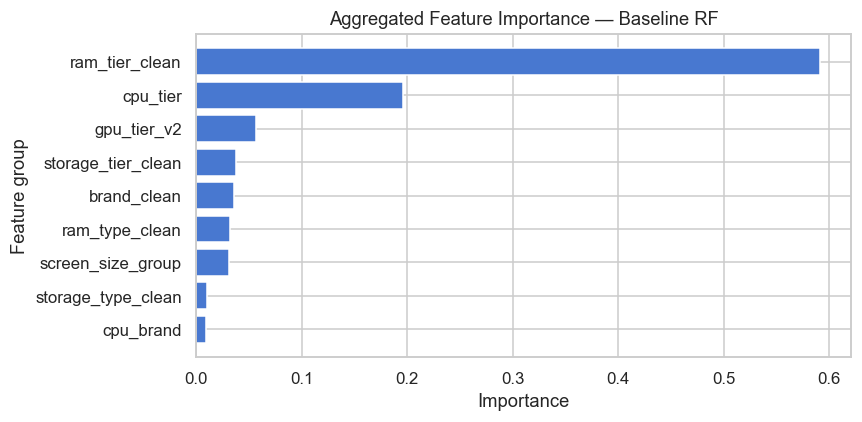
\includegraphics[width=0.7\textwidth]{images/websach_img_21.png}
    \caption{Kết quả dự đoán giá của baseline Random Forest trên Websosanh. Mô hình đạt $R^2 = 0.746$ nhưng có sai số lớn ở nhóm high-end.}
    \label{fig:baseline-results}
\end{figure}
